%!TEX root = presentazionelancia.tex

\setlength{\parskip}{\baselineskip} 
\section*{Introduction}
\begin{frame}[t]
\frametitle{Introduction}
\begin{block}{What is TAO?}
	TAO is a geographically distribute store
	\begin{itemize}
		\item deployed at Facebook
	 	\item with efficient and timely access to social graph
	 	\item using a fixed set of query
	 	\item replacing memcache
	 	\item running on thousands of machines
	 	\item provide access to many PB of data
	 	\item process a billion reads ad millions of writes each second!
	 \end{itemize} 
\end{block}
\end{frame}

\begin{frame}
\frametitle{The social graph}
Facebook has more than 1 billion active user 
\begin{itemize}
	\item recording relationships,
	\item sharing interests,
	\item uploading pictures and \dots
\end{itemize}

The user experience of Fb comes from rapid, efficient and scalable access to the \emph{social graph}
\end{frame}

\begin{frame}
	What's behind an entry in yours Fb page?

	\begin{center}
	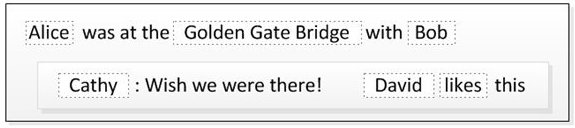
\includegraphics[width=0.8\textwidth]{figs/social.jpg}	\\
	\end{center}
	A single Fb page aggregate and filter hundreds of items from the social graph.
\end{frame}%

\begin{frame}[t]
\begin{center}
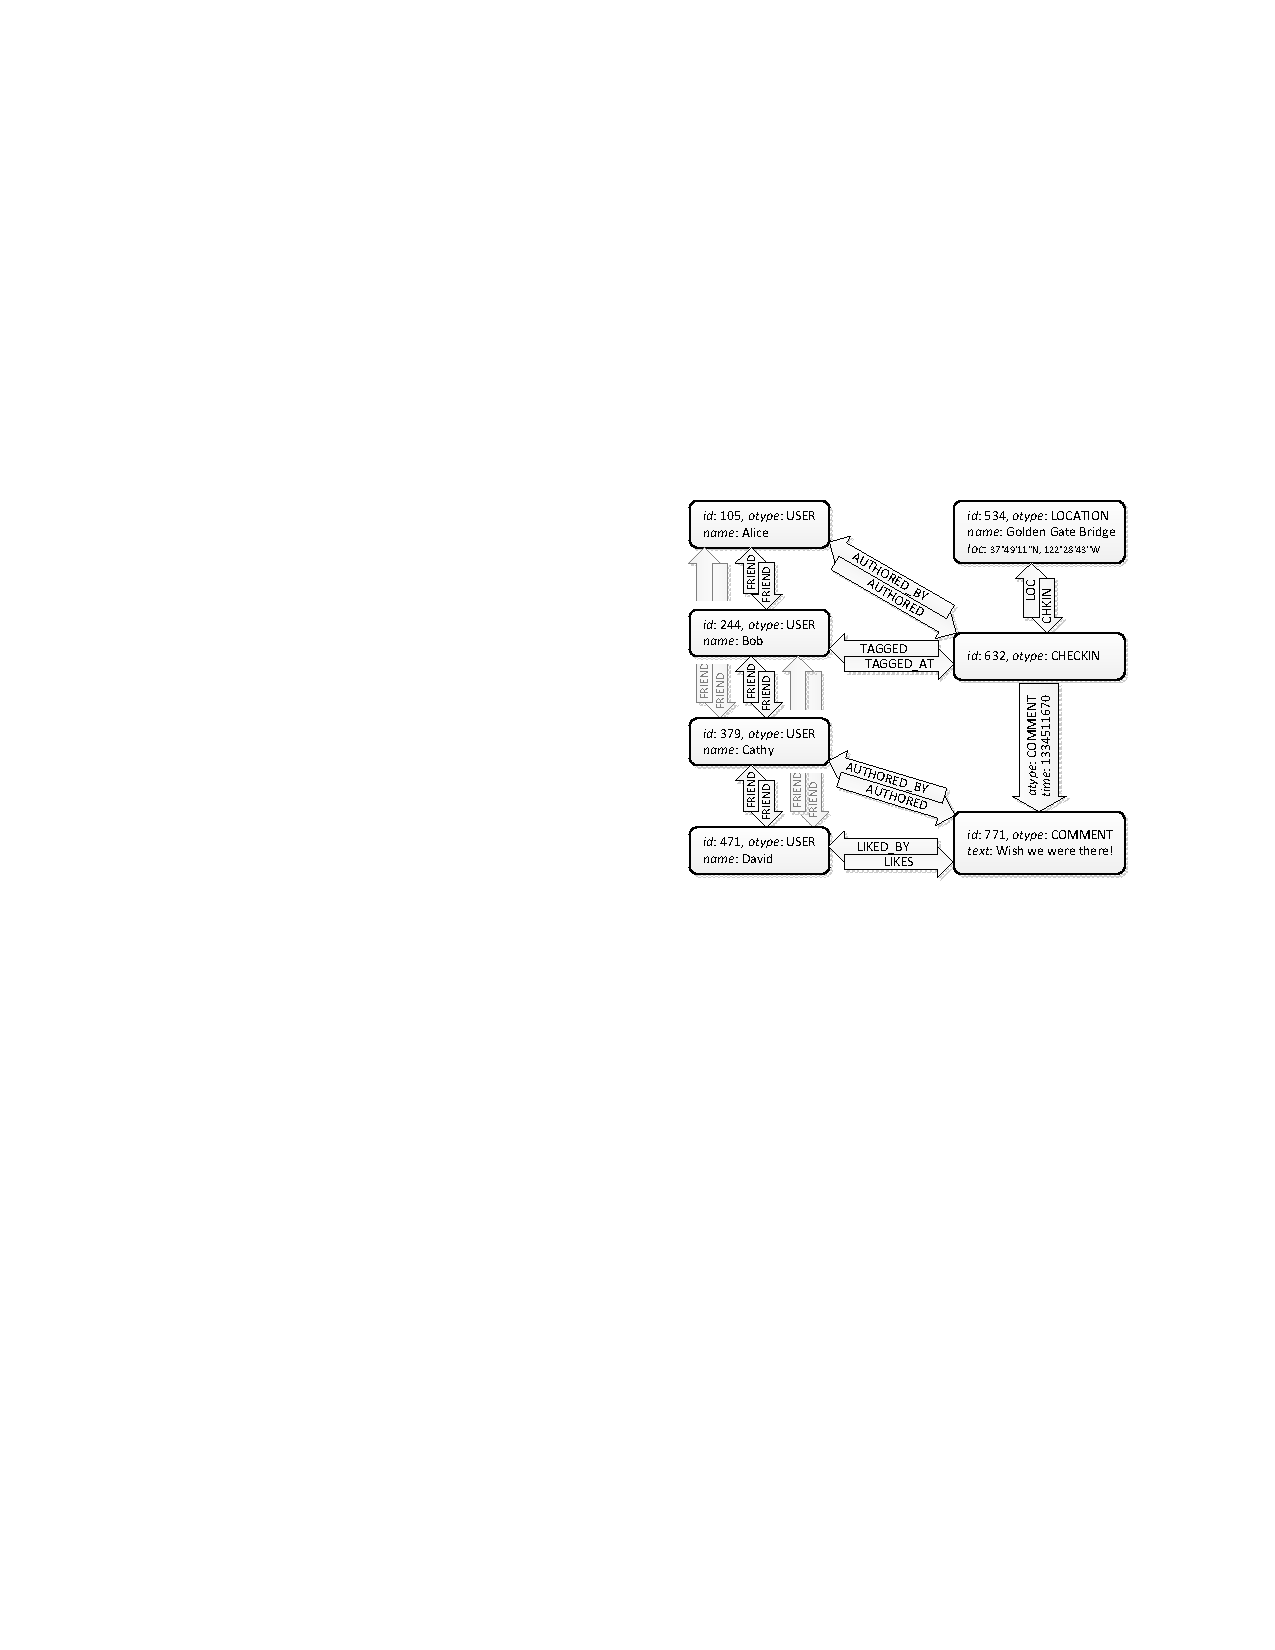
\includegraphics[width=0.8\textwidth]{figs/social2}	
\end{center}


\end{frame}

\begin{frame}
\frametitle{Before Tao}
	\begin{itemize}
 	\item Facebook was storing the social graph to MySql
	\begin{itemize}
		\item  	Quering it from PHP
		\item  	Storing result in memcache\\
	\end{itemize}
	\end{itemize}
	\begin{center}
		
\includegraphics[width=0.3\textwidth]{figs/php-logo.eps}\quad
		
\includegraphics[width=0.3\textwidth]{figs/mysql.png}
	\end{center}
 	Over time Fb deprecated direct access to MySQL in favor of a graph (associations, nodes) abstraction
\end{frame}

\begin{frame}
\frametitle{Limits}
    \begin{itemize}
    	\item Operations on lists are inefficient in memcache (update whole list)
    	\item Complexity on clients managing cache
    	\item Hard to offer read-after-write consistency
    \end{itemize}
Also they want to access social graph from non-PHP services
\end{frame}

\begin{frame}
\frametitle{TAO's Goals}
	\begin{itemize}
		\item Efficiency at Scale
		\pause
		\item Low read latency
		\pause
		\item Timeliness of writes
		\pause
		\item High read availability
	\end{itemize}
\end{frame}
